\DiaryEntry{Polynomials, 3 (Quotient Rings)}{2016-08-09}{Algebra}

\subsection{Ideals (Repetition)}\label{ideals-repetition}

An ideal \(I = \langle a \rangle\) is defined as
\(I = \langle a \rangle = \{a b, b\in \mathbb{Z} \}\). As an example,
consider \(I = \langle 2 \rangle = \{\ldots, -4,-2,0,2,4,\ldots\}\). The
elements are a subset of \(\mathbb{Z}\); i.e.~every second element of
\(\mathbb{Z}\).

\begin{figure}[H]
\centering
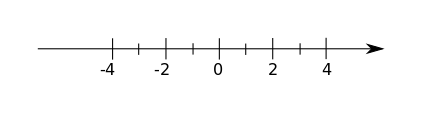
\includegraphics{images/polynomials_03.png}
\caption{Page1}
\end{figure}

Cosets are ``shifted'' ideals; e.g. \(J+1\) is the ideal shifted by one:
\(J+1 = \{\ldots,-3,-1,1,3,\ldots\}\). The set of all cosets cover the
complete \(\mathbb{Z}\). Cosets are either disjoint or contain the same
elements. In this case it is rather obvious when two cosets are disjoint
(e.g.~J and J+1) or contain the same elements (e.g.~J and J+2).

\subsection{\texorpdfstring{The Field
\(\mathbb{Z}[x] / \langle p(x) \rangle\)}{The Field \textbackslash{}mathbb\{Z\}{[}x{]} / \textbackslash{}langle p(x) \textbackslash{}rangle}}\label{the-field-mathbbzx-langle-px-rangle}

Let p(x) be a polynomial with coefficients from \(\mathbb{Z}\);
therefore the polynomial is from \(\mathbb{Z}[x]\). In the extension
field topic, \(p(x)\) has a root: \(p(\alpha) = 0\).

\(J = \langle p(x) \rangle\) is the ideal; i.e.~all polynomials of the
form \(a(x)p(x), a(x) \in \mathbb{Z}[x]\). Note that all elements of the
ideal have \emph{at least} the root \(\alpha\) (the \(a(x)\) may
introduce other roots as well).

If we choose \(p(x) = x^2-2\), then
\(J = \{ \ldots, x^2-2, x(x^2-2), (x+1)(x^2-2), \ldots \}\). Somewhat
unintuitively, \(J\) does \emph{not} contain \emph{all} polynomials of
\(\mathbb{Z}[x]\) (similar to the ideal \(\langle 2 \rangle\));
e.g.~polynomials of degree 0 and 1 are not contained in J.

A coset \(J + a\) is defined as
\(\{j + a, j \in J, a \in \mathbb{Z} \}\) for fixed \(a\) and \(j\)
ranging over the whole ideal J. Note that the cosets are disjoint sets
(i.e. \(J+a\) and \(J+b\) are disjoint for \(a \neq b\)) and partition
\(\mathbb{Z}\). In our example, the coset \(J + -(x^2-2)\) will contain
the constant polynomial \(1\). While for the cosets of the ideal
\(I = \langle 2 \rangle\) it was obvious which cosets are disjoint and
which contain the same elements, this is not obvious in this example.

The quotient ring is the set of all cosets; i.e.
\(\mathbb{Z} / \langle p(x) \rangle = \{\ldots, J - x, J-2x, J, J+x^2, J+2x^2,\ldots\}\).
This quotient ring forms a field.
